It is not surprising that weather conditions directly impact the wind power generation. The typical input parameters for wind power prediction are wind speed, air density, temperature and pressure \cite{WindPowerGenerationUsingANN} with the most influential factor being wind speed because it is directly converted to power in the wind turbine. The following subsections will describe the parameters relationship to wind production and how it is used in the modelled ANN.

The Pearson Correlation Coefficient\footnote{\url{http://en.wikipedia.org/wiki/Pearson_product-moment_correlation_coefficient}} has been used to establish the linear dependency between meteorological factors, consumption and wind production. Table ~\ref{table:pearsonCoeficientWindProduction} shows this correlation coefficient. The factors have been discussed throughout the thesis as having an influence on the wind speed production to some degree. The Pearson Correlation Coefficient returns a value between -1 and +1 which indicates the strength of the linear correlation between two variables.

\begin{table}[H]
\centering  % used for centering table
\begin{tabular}{c c} % centered columns (3 columns)
Input factor \#1 & Pearson Correlation Coefficient \\ [0.5ex] % inserts table 
%heading
\hline                  % inserts single horizontal line
Consumption & 0.61526858399 \\ % inserting body of the table
Wind Speed & 0.93199144444 \\
Temperature & -0.0924058954431 \\
Wind Direction & 0.191866256937 \\ [1ex] % [1ex] adds vertical space
\hline %inserts single line
\end{tabular}
\caption{Table showing Pearson correlation coefficient between various factors and the wind production.} % title of Table
\label{table:pearsonCoeficientWindProduction} % is used to refer this table in the text
\end{table}

\subsubsection{Wind Speed}
The relationship between hourly wind speed and hourly wind power production of DK1 is seen in Figure~\ref{fig:windVsProd}. The graph clearly shows the expected impact of wind speed on the wind energy production.

\begin{figure}[H]
\centering
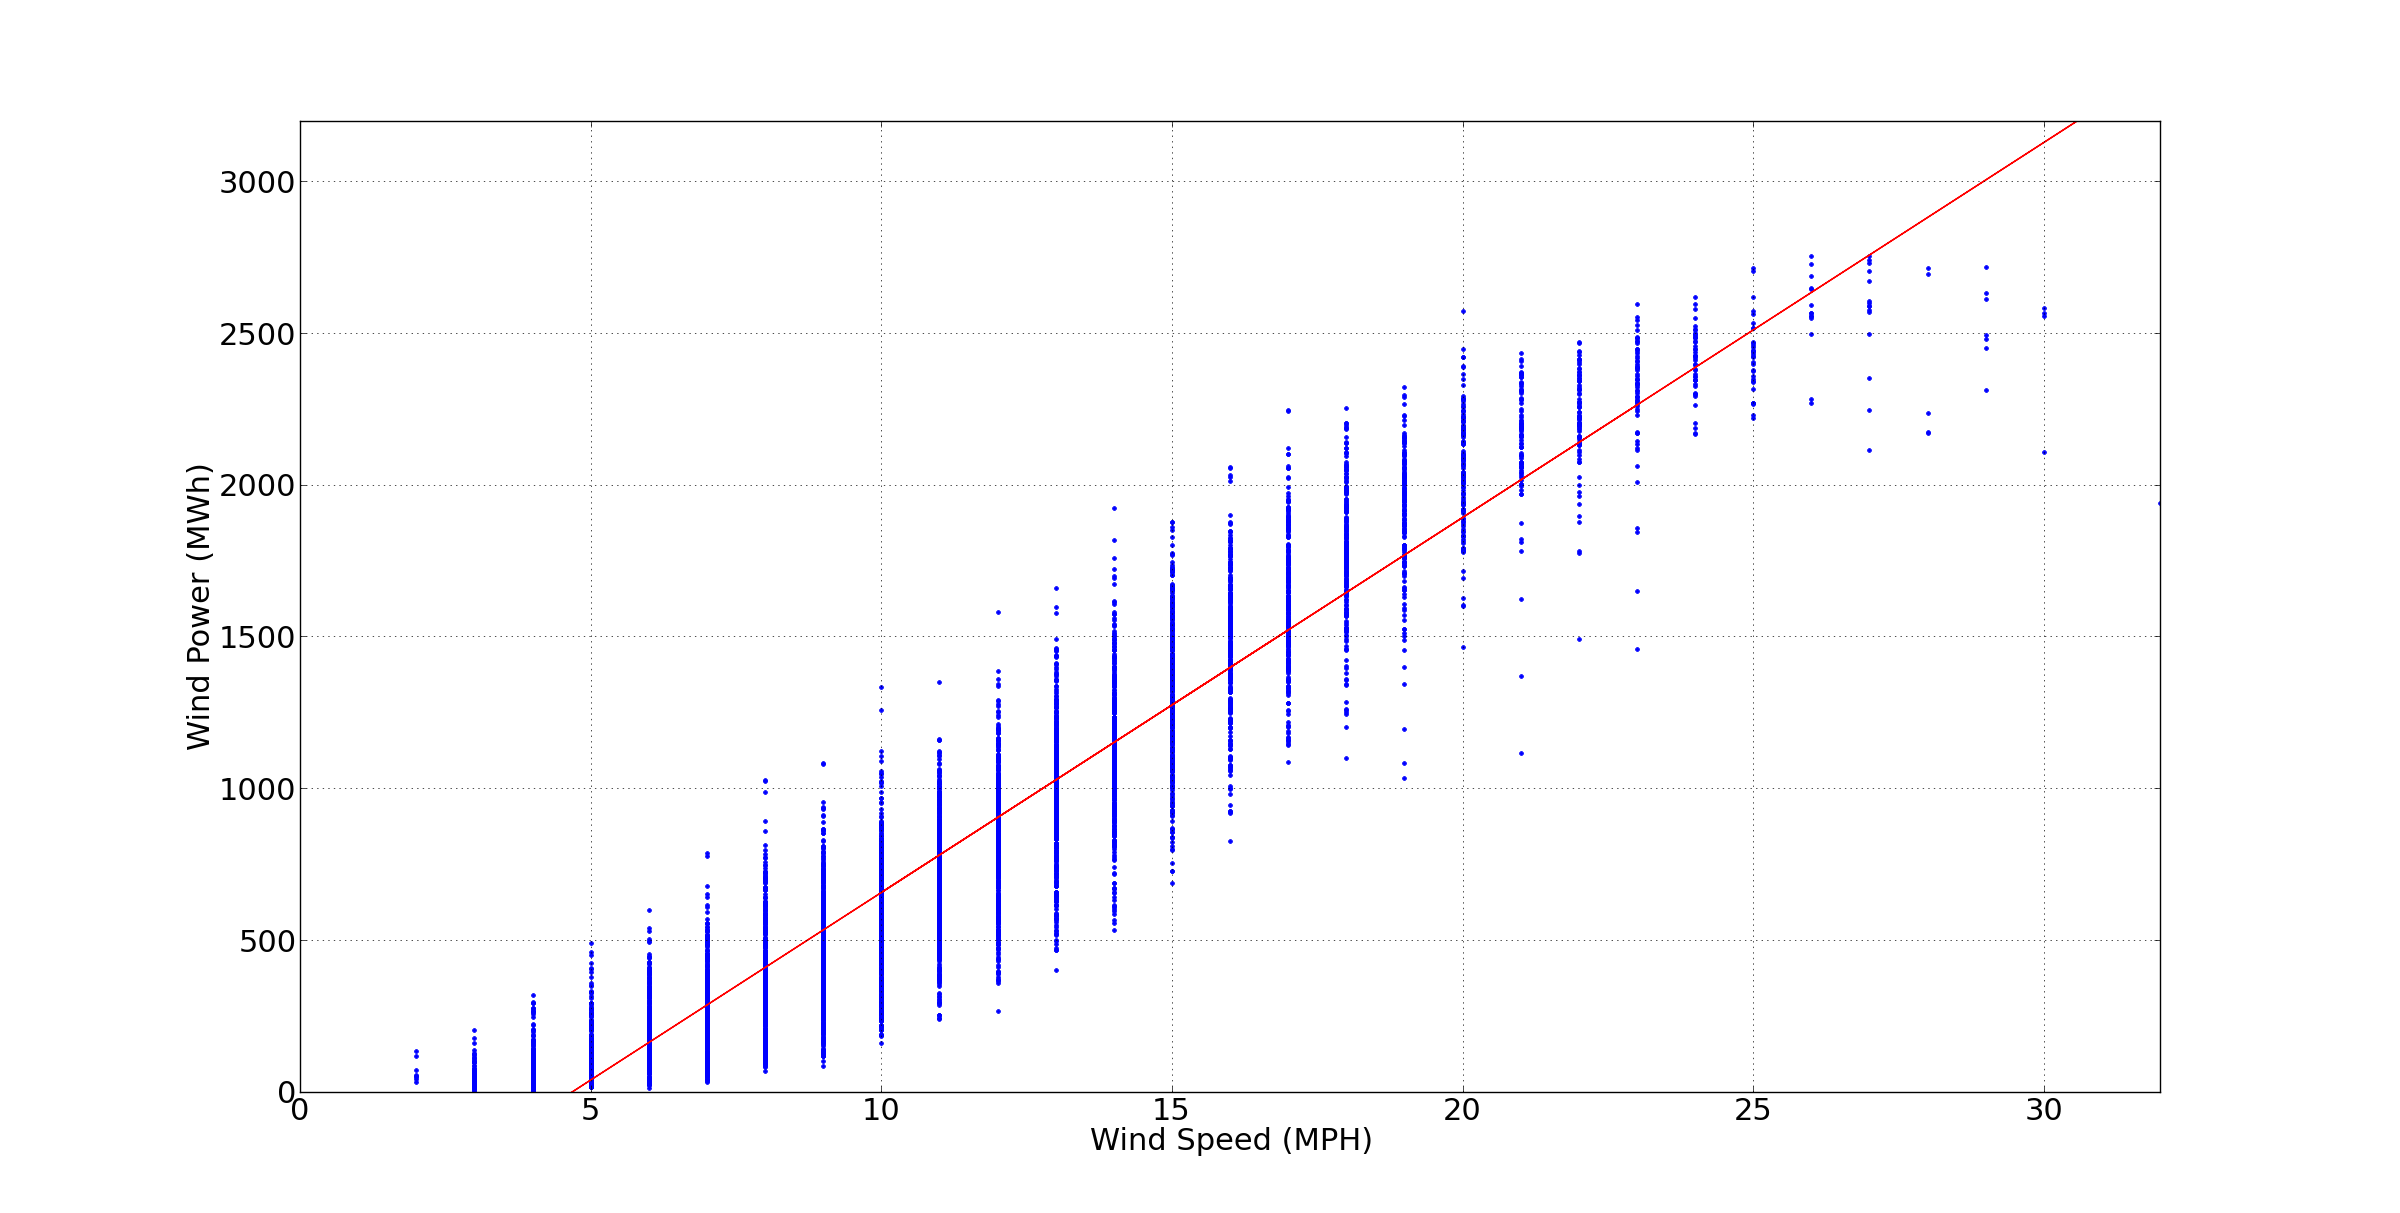
\includegraphics[width=0.99\linewidth,natwidth=898,natheight=587]{billeder/WindSpeedVsProduction.png}
\caption{Wind speed vs. wind production in 2012}
\label{fig:windVsProd}
\end{figure}

\subsubsection{Air Density}
It is described in the Wind Power Production section that wind energy is proportional to air density where a higher density means more power for a specific wind speed. This does not imply that a higher air density is equal to higher wind power production in general because it depends on the wind speed. Days with equal wind speed but variation in air density should show an increase in power production when the air density is highest. 

Air density depends directly on temperature and pressure which can be described by $Air Density=\frac{P*M}{(R*T)}$ where R is a gas constant and M is the density of air. The monthly pressure in Denmark has low variation compared to the temperature as shown in Figure~\ref{fig:pressureTemperatureVariance}. For this reason, the temperature will have the most influence on the air density in Denmark. The formula express that when temperature decreases the air density will increase linearly, e.g. the wind power production for a specific wind speed will be higher in times of low temperature. This exact relationship is seen in some statistics that i will do IN A FIGURE HERE1.
The air density has been calculated for every hour in the training set and the result can be seen in Figure~\ref{fig:windProductionVsAirDensity}. The relationship is as expected and the power production increases with the air density.

\begin{figure}[H]
\centering
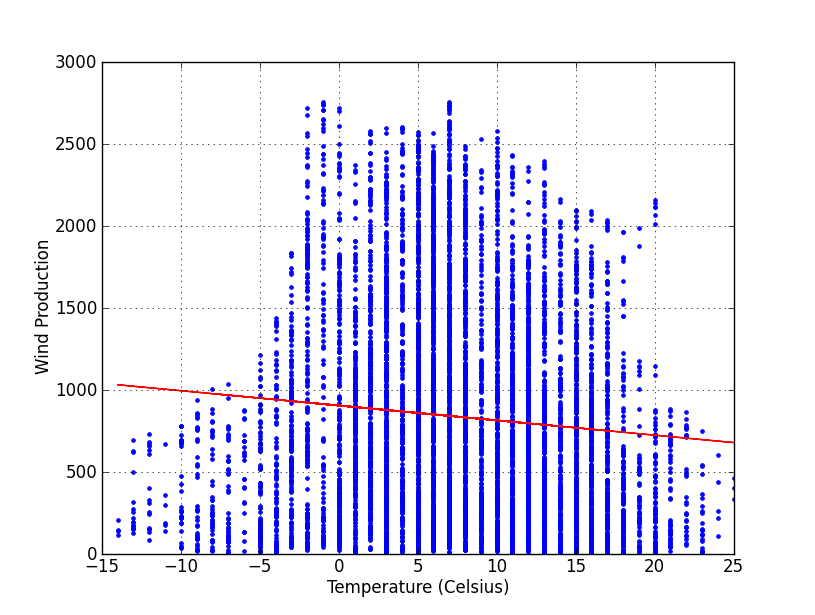
\includegraphics[width=0.99\linewidth,natwidth=898,natheight=587]{billeder/tempVsProd.png}
\caption{Temperature and Pressure variance for 2012}
\label{fig:tempVsProd}
\end{figure}

\begin{figure}[H]
\centering
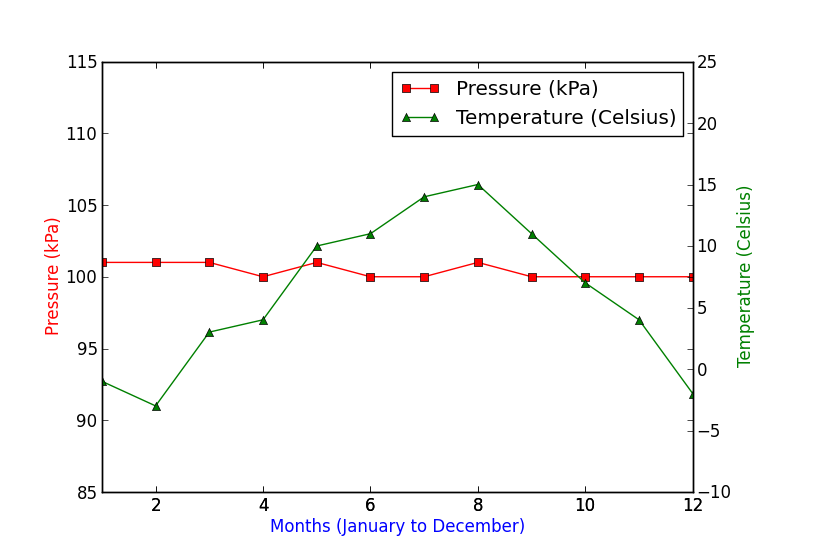
\includegraphics[width=0.99\linewidth,natwidth=898,natheight=587]{billeder/pressureTemperatureVariance.png}
\caption{Temperature and Pressure variance for 2012}
\label{fig:pressureTemperatureVariance}
\end{figure}

\begin{figure}[H]
\centering
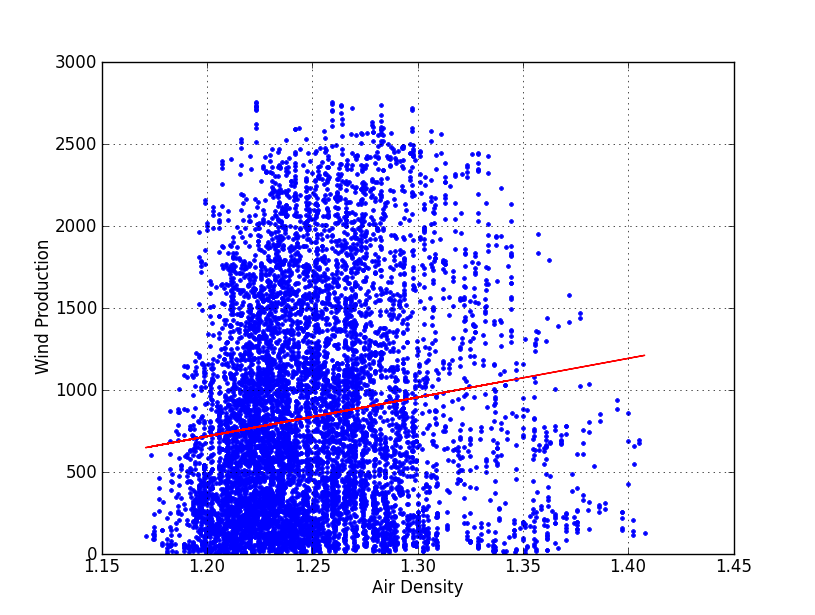
\includegraphics[width=0.99\linewidth,natwidth=898,natheight=587]{billeder/windProductionVsAirDensity.png}
\caption{Air Density vs. Wind Power in 2012}
\label{fig:windProductionVsAirDensity}
\end{figure}

\subsubsection{Wind Direction}
bla bla intro. Figure~\ref{fig:windDirVsProd} shows that western wind has a tendency to produce more energy. (need to further investigated but seems valid when looking at dk).
\begin{figure}[H]
\centering
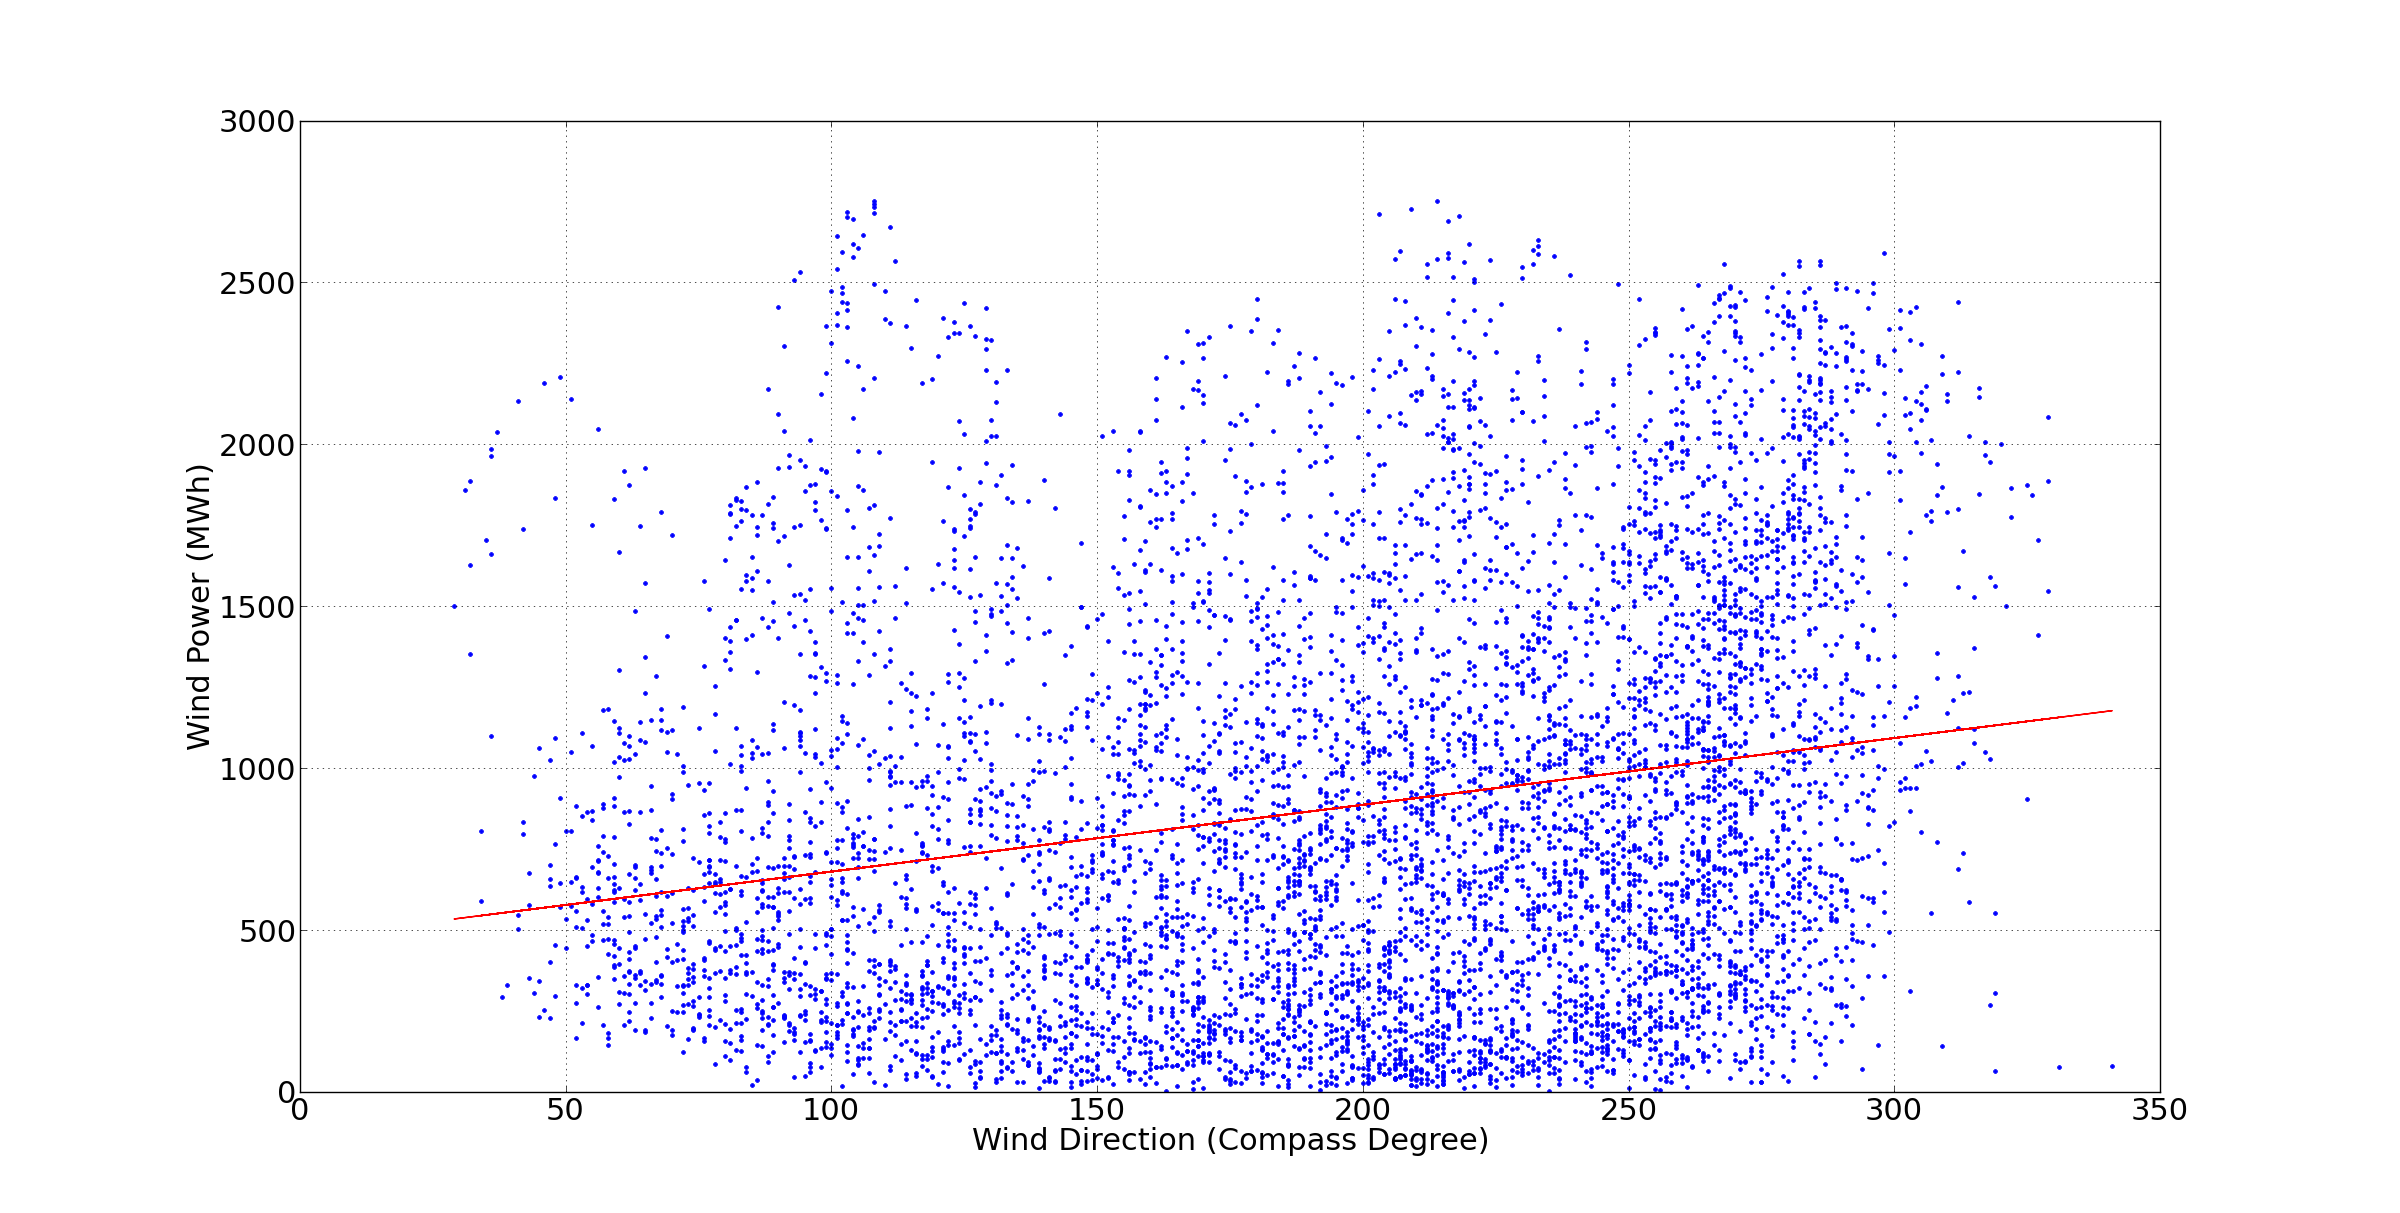
\includegraphics[width=0.99\linewidth,natwidth=898,natheight=587]{billeder/productionVsWindDirection.png}
\caption{Wind Direction vs. wind production in 2012}
\label{fig:windDirVsProd}
\end{figure}

\subsubsection{Consumption}
It is expected that the wind power available on the energy market will be low at times with low consumption, e.g if no energy is needed the wind power can't be sold.  This relationship is shown in Figure~\ref{fig:consumptionVsWindProduction}.

\begin{figure}[H]
\centering
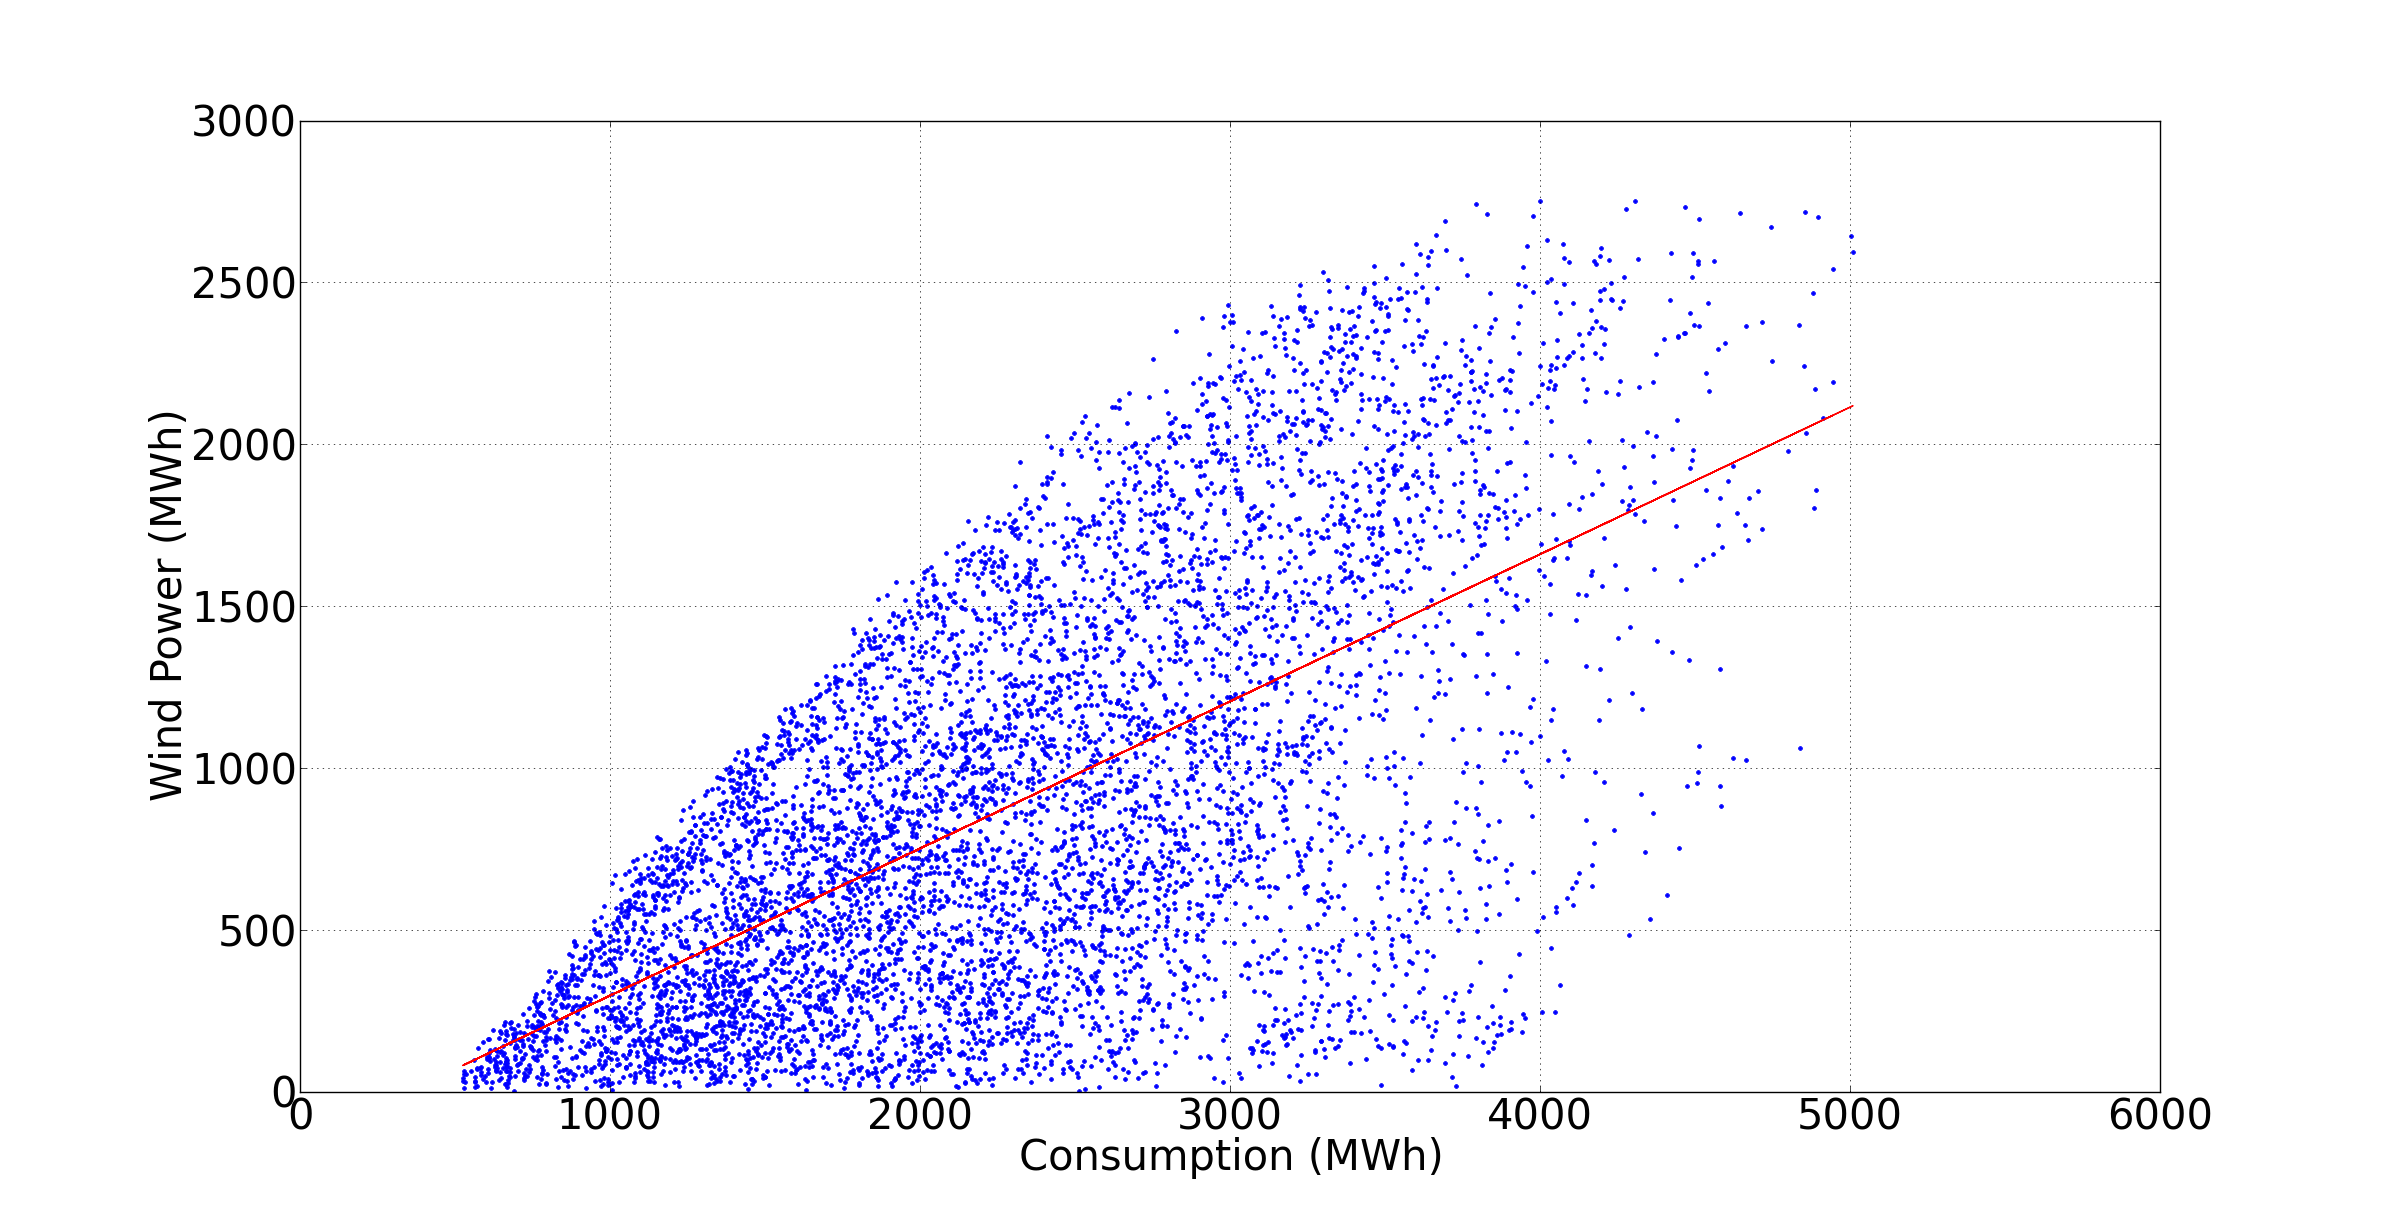
\includegraphics[width=0.99\linewidth,natwidth=898,natheight=587]{billeder/consumptionVsWindProduction.png}
\caption{Consumption vs. Wind Production in 2012}
\label{fig:consumptionVsWindProduction}
\end{figure}

\subsection{Modelling Artificial Neural Network}
The ANN will be trained with input the hourly parameters of wind speed, temperature, pressure and humidity and then compared to the actual production of that hour.

Black art --- experimenting with hidden layers, momentum and learning rate. 